\subsection{E5: the separation inside a trained network}
\label{sec:res-e5}

Table~\ref{tab:e5} and Fig.~\ref{fig:e5} report the diagnostic applied to the
compressed-computation models. Three findings stand out; one of them we did not anticipate, and
one prediction we had made was not borne out.

\paragraph{The $L^4$-trained network attains the floor.} Its calibrated linear interface has
attainment ratio \EfiveLfourRatioPinvMean{} under the pseudoinverse readout (range
$[\EfiveLfourRatioPinvMin,\EfiveLfourRatioPinvMax]$ over \EfiveSeeds{} seeds) and
\EfiveLfourRatioLsMean{} under the fitted least-squares readout (range
$[\EfiveLfourRatioLsMin,\EfiveLfourRatioLsMax]$), against a floor of $W=\EfiveWelchFloor$. The
$L^2$ baseline sits at \EfiveLtwoRatioLsMean{} and the random-code control at
\EfiveRandRatioLsMean. E4 had shown the floor to be reachable by direct optimisation of the
cross-talk; here it is approached by a network optimising a task loss that never mentions
interference.

Two caveats on the statistics, both cutting against reading too much into them. First, the
comparison with the random code is readout-dependent: $L^4$ is closer to the floor than an
i.i.d.\ code of the same shape under the pseudoinverse (\EfiveLfourRatioPinvMean{} versus
\EfiveRandRatioPinvMean) and under least squares, but its own trained decoder is
\emph{farther} from the floor (\EfiveLfourRatioWoutMean) than either. That last figure has no
counterpart in the control and we do not pair it with one: the random code has no trained
decoder, so its $W_{\mathrm{out}}$ column is by construction the pseudoinverse and would be
compared against a different object. Across the readouts that do admit a matched comparison,
the trained code is comparable to a random one on this axis, not better. Second, every pairwise test returns
$p=\EfiveMwPLfourLtwo$ with $|\delta|=1$, which is exactly the smallest two-sided $p$ an exact
Mann--Whitney can produce at $n=\EfiveSeeds$ per group: within-group variance is negligible, so
the test reports ``no overlap'' and nothing more. The effect sizes are what separate the cases,
and they differ by orders of magnitude --- \EfiveLtwoRatioLsMean{} versus
\EfiveLfourRatioLsMean{} for $L^2$ against $L^4$, a few percent for $L^4$ against random. No
multiplicity correction is applied across the nine tests, and at this $n$ none would survive
one.

\paragraph{The separation is real but much narrower than we predicted, and the $s_{95}$
statistic runs against us.} Our pre-registered expectation was that the network's thresholded
output would remain exact over a strictly wider sparsity range than its best linear readout.
The measurement contradicts that at the sparsities where both work. Ranking the three linear
readouts by exact-recovery rate at each $s$ and taking the best of them, the network is behind
up to $s=4$: at $s=3$ both are exact, and at $s=4$ the network recovers in
\EfiveLfourPmodelFour{} of trials while the calibrated $W_{\mathrm{out}}$ interface recovers in
\EfiveLfourPlinFour. On the $s_{95}$ statistic the linear readout is strictly ahead --
$s_{95}=\EfiveLfourSlinBestMax$ against the network's \EfiveLfourSmodelMax{} on all
\EfiveSeeds{} seeds at $p=\EfivePrimaryP$, and ahead on
\EfiveLfourSlinAheadSecondary{} of \EfiveSeeds{} seeds (tied on the remainder) at
$p=\EfiveSecondaryP$ (Table~\ref{tab:e5}). The preregistered comparison is not supported.

The network only leads further out, where both decoders are already unreliable: at $s=5$,
\EfiveLfourPmodelFive{} versus \EfiveLfourPlinFive, and at $s=6$, \EfiveLfourPmodelSix{} versus
\EfiveLfourPlinSix. E5 therefore shows the network extending the usable sparsity range past the point where the
thresholded linear readouts of its own code have collapsed, not dominating them everywhere.

The floor statement is on firmer ground, but it is worth being exact about what it is. At every
sparsity analog reconstruction carries irreducible error: at $s=3$, where the network is exact in
\EfiveLfourPmodelThree{} of trials, the best linear readout still has per-coordinate RMS error
\EfiveLfourRmsThree{} against its floor of \EfiveLfourFloorThree. That non-zero error is
Theorem~\ref{thm:floor} restated for this code, not an independent measurement --- any
rank-$d$ unit-diagonal interface has it by construction. What E5 measures is its \emph{size} for
a code that gradient descent actually produced, and how far the thresholded decoder gets before
that error stops it.

\paragraph{The $L^2$ model is maintaining a linear interface.} This is the finding we did not
plan for. In the $L^2$ models the ReLU is active on only \EfiveLtwoNegPre\% of preactivations,
the learned decoder sits at relative distance \EfiveLtwoWoutPinvDist{} from the pseudoinverse of
the encoder, and the network's thresholded decision agrees with that of a plain linear readout
on \EfiveLtwoAgreeLinear\% of evaluation states. The $L^4$ models are elsewhere: ReLU active on
\EfiveLfourNegPre\% of preactivations, decoder at relative distance \EfiveLfourWoutPinvDist,
and agreement with the linear readout down to \EfiveLfourAgreeLinear\%. The diagnostic thus
reproduces, from interface measurements alone and without any mechanistic reverse-engineering,
the distinction that~\cite{bhagat2026cc} and~\cite{ferreiradasilva2026l4} reached by other
means. It also explains why the $L^2$ model is bound by Theorem~\ref{thm:floor} at all: a
network that keeps an effectively linear readout \emph{is} a linear readout for these inputs,
and its measured ratio of \EfiveLtwoRatioLsMean{} says how far from optimal that readout is.
Its thresholded output recovers even a single active feature only \EfiveLtwoPmodelOne{} of the
time.

\paragraph{The finding replicates at a second training sparsity.} Everything above is measured
at $p=\EfivePrimaryP$. Repeating the whole campaign at $p=\EfiveSecondaryP$ (ablation A5,
\EfiveSeeds{} fresh seeds per condition) reproduces both halves: the $L^4$ models sit at
\EfiveLfourSecRatioLsMean{} against the floor and agree with a linear readout on only
\EfiveLfourSecAgreeLinear\% of states, while the $L^2$ models sit at
\EfiveLtwoSecRatioLsMean{} and agree \EfiveLtwoSecAgreeLinear\% of the time. The interface
distinction is therefore not an artefact of one input sparsity.

\paragraph{What does not favour our hypothesis.} Three things. The $L^4$ models have a
\emph{worse} mean squared error on the training task than the $L^2$ models (\EfiveLfourMse{}
versus \EfiveLtwoMse), as expected since they optimise a different objective: the interface
advantage is not a task-performance advantage, and we do not claim it is. The $s_{95}$
prediction above failed. And the random-code control is a reminder that a good interface is not
by itself evidence of computation: its \emph{linear} readout recovers exactly with probability
\EfiveRandPlinThree{} at $s=3$, better than the $L^2$ network, simply because an i.i.d.\ code is
already near-Welch-optimal (ratio \EfiveRandRatioLsMean). What the random control lacks is the
nonlinear stage; the ``network'' column for that row is not meaningful and is reported only for
completeness.

\begin{figure}[t]
\centering
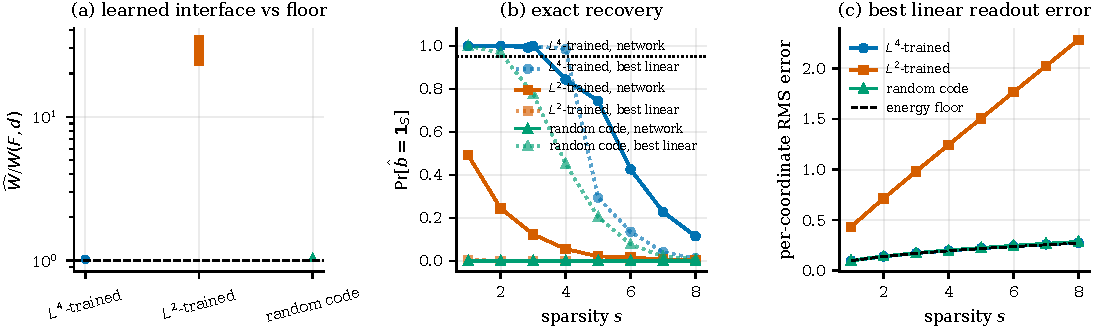
\includegraphics[width=\linewidth]{figures/fig3_trained_model.pdf}
\caption{\textbf{Interface separation inside a trained toy model of computation in
superposition.} A width-\EfiveD{} network trained to compute \EfiveF{} sparse ReLU features
(setup of~\cite{braun2025apd}; $L^4$ variant of~\cite{ferreiradasilva2026l4}); one point per
seed. (a) Attainment ratio of the learned calibrated interface against the floor of
Theorem~\ref{thm:floor}. (b) Exact recovery by the network's thresholded output (solid) versus
the best linear readout of the same code (dotted). (c) Per-coordinate RMS error of the best
linear readout against the energy floor of Proposition~\ref{prop:uniform-energy}. Generated by
\code{scripts/make\_figures.py} from \code{results/e5}.}
\label{fig:e5}
\end{figure}

\begin{table}[t]
\centering
\caption{E5: the diagnostic applied to trained models, averaged over \EfiveSeeds{} seeds at
training sparsity $p=\EfivePrimaryP$. ``Agrees with linear'' is the fraction of evaluation
states on which the network's thresholded decision coincides with that of a plain linear
readout --- the quantity that identifies which interface the model maintains.}
\label{tab:e5}
\small
% Generated by scripts/make_tables.py from results/. Do not edit by hand.
\begin{tabular}{lrrrrr}
\toprule
model & $\widehat{W}/W$ & $s_{95}$ (network) & $s_{95}$ (best linear) & ReLU clipped (\%) & agrees with linear (\%) \\
\midrule
$L^4$-trained & 1.022 & 3.0 & 4.0 & 48.6 & 21.8 \\
$L^2$-trained & 28.814 & 0.0 & 0.0 & 4.6 & 99.1 \\
random code & 1.055 & 0.0 & 2.0 & 50.0 & 13.8 \\
\bottomrule
\end{tabular}

\end{table}

\subsubsection*{What the attainment ratio was measuring}
\label{sec:res-g1}

The ratios above are referenced to $W(F,d)$, and Section~\ref{sec:codefloor} showed that such a
ratio conflates two questions. Applying the factorisation~\eqref{eq:decomposition} to the same
models settles which of the two the reported numbers answered, and the answer is uncomfortable:
one of them, entirely.

Under the calibrated pseudoinverse the readout factor is $1$ to six decimals in every cell ---
\GoneLfourRreadoutPinv{} for $L^4$, \GoneLtwoRreadoutPinv{} for $L^2$,
\GoneRandRreadoutPinv{} for the random control --- which is not a measurement but
Theorem~\ref{thm:codefloor} restated, since the calibrated pseudoinverse \emph{is} the
code-specific optimum. The whole ratio is therefore $R_{\mathrm{geom}}$:
\GoneLfourRgeom{} against a reported \GoneLfourRatio{} for $L^4$, \GoneLtwoRgeom{} against
\GoneLtwoRatio{} for $L^2$, \GoneRandRgeom{} against \GoneRandRatio{} for the random code. So
the claim that the $L^4$ model comes ``within a few parts in a thousand of the floor'' is a
statement about the evenness of its leverage profile, and contains no information about its
decoder. We restate it that way.

Asking the decoder question separately reverses the ordering. Measured against the best readout
of its \emph{own} code, the $L^4$ network's trained output layer sits at
$R_{\mathrm{readout}}=\GoneLfourRreadoutWout{}$ while the $L^2$ network's sits at
\GoneLtwoRreadoutWout{} --- so on this criterion the $L^2$ model has the better decoder and the
worse code, the opposite of the reading the single ratio invites. The random control's own
readout gives exactly \GoneRandRreadoutWout{}, which is a consistency check rather than a
finding: that baseline sets $W_{\mathrm{out}}=\Phi^{+}$ by construction, so its ``own decoder''
is the code-specific optimum by definition, and any other value would indicate a bug.

The mechanism is visible in the leverage profiles, and it is the quantity
Corollary~\ref{cor:failthresh} needs. The $L^4$ code spreads leverage almost uniformly, from
\GoneLfourLeverageMin{} to \GoneLfourLeverageMax{} with coefficient of variation
\GoneLfourLeverageCv{}; the random code is comparable at \GoneRandLeverageMin{} to
\GoneRandLeverageMax{} (coefficient of variation \GoneRandLeverageCv{}); the $L^2$ code is not,
running from \GoneLtwoLeverageMin{} to \GoneLtwoLeverageMax{} with coefficient of variation
\GoneLtwoLeverageCv{}. That dispersion is exactly the excess of Proposition~\ref{prop:excess},
and it grows with the training density: at $p=0.02$ the $L^2$ geometry factor rises to
\GoneLtwoRgeomDenseP{}.

Two limits on what this licenses. The factorisation is arithmetic on
Theorem~\ref{thm:codefloor} and needs no new assumption, but it reinterprets an existing
measurement rather than adding evidence --- five seeds at one width remain five seeds at one
width. And \GoneLtwoLeverageMin{} is the number Corollary~\ref{cor:failthresh} consumes: with
$s=2$ the threshold $\min\{\tfrac12,(s-1)^2/((F-1)+(s-1)^2)\}$ is exactly $1/F$, so at
$F=\EfiveF$ it is $0.01$, and the measured minimum leverage of the $L^2$ code falls below it. The
theory therefore predicts that this code loses affine separability at $s=2$ --- from a single
leverage score, with no decoder and no probe in the argument. The corollary is applied at the
minimum leverage, which is where it is strongest and, being below a half, also where its
hypothesis holds. Whether that prediction survives at other widths is the
question Section~\ref{sec:limitations} flags as open.

